\documentclass[border=15pt, multi, tikz]{standalone}
%\usepackage{blocks}
\usepackage{import}
\subimport{../../layers/}{init}
\usetikzlibrary{positioning}
\usetikzlibrary{3d}

\def\ConvColor{rgb:yellow,5;red,2.5;white,5}
\def\ConvReluColor{rgb:yellow,5;red,5;white,5}
\def\ResizeColor{rgb:green,1;black,1}
\def\PoolColor{rgb:red,1;black,0.3}
\def\FcColor{rgb:blue,5;red,2.5;white,5}
\def\FcReluColor{rgb:blue,5;red,5;white,4}
\def\SoftmaxColor{rgb:magenta,5;black,7}

\begin{document}
\begin{tikzpicture}
\Large
\tikzstyle{connection}=[ultra thick,every node/.style={sloped,allow upside down},draw=\edgecolor,opacity=0.7]
%%%%%%%%%%%%%%%%%%%%%%%%%%%%%%%%%%%%%%%%%%%%%%%%%%%%%%%%%%%%%%%%%%%%%%%%%%%%%%%%%%%%%%%%
%% Draw Layer Blocks
%%%%%%%%%%%%%%%%%%%%%%%%%%%%%%%%%%%%%%%%%%%%%%%%%%%%%%%%%%%%%%%%%%%%%%%%%%%%%%%%%%%%%%%%
\node[canvas is zy plane at x=0] (temp) at (-3,-2,0) {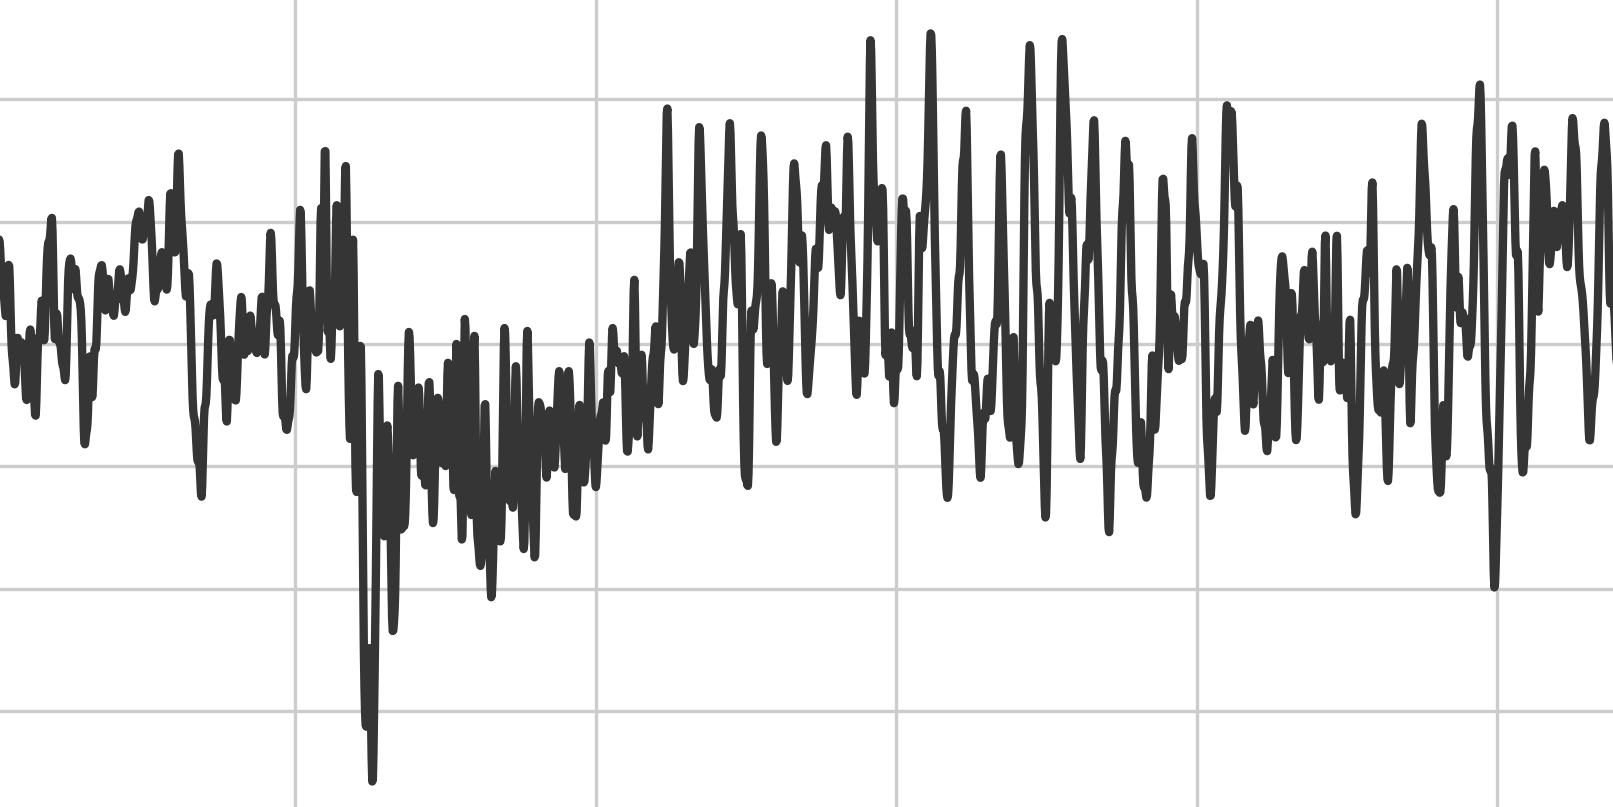
\includegraphics[width=18cm,height=3cm]{signal.png}};

%transp conv1
\pic[shift={(0,0,5)}] at (0,0,0) {RightBandedBox={name=tc1,caption=tc1,%
	xlabel={{32,}},ylabel=4,zlabel=\Large{2700},fill=\ConvColor,bandfill=\ConvReluColor,%
	width=14,height=8,depth=96}};

%transp conv2
\pic[shift={(2,0,0)}] at (tc1-east) {RightBandedBox={name=tc2,caption=tc2,%
	xlabel={{16,}},ylabel=13,zlabel=\Large{2700},fill=\ConvColor,bandfill=\ConvReluColor,%
	width=10,height=14,depth=96}};

%resize1
\pic[shift={(2,0,0)}] at (tc2-east) {Box={name=rz1,caption=rz1,%
	xlabel={16,},ylabel=116,zlabel=\Large{1809},fill=\ResizeColor,opacity=0.5,%
	width=10,height=30,depth=88}};

% transp conv3
\pic[shift={(2,0,0)}] at (rz1-east) {RightBandedBox={name=tc3,caption=tc3,%
	xlabel={{8,}},ylabel=117,zlabel=\Large{1809},fill=\ConvColor,bandfill=\ConvReluColor,%
	width=7,height=30,depth=88}};

% transp conv4
\pic[shift={(2,0,0)}] at (tc3-east) {RightBandedBox={name=tc4,caption=tc4,%
	xlabel={{8,}},ylabel=235,zlabel=\Large{1809},fill=\ConvColor,bandfill=\ConvReluColor,%
	width=7,height=38,depth=88}};

%resize2
\pic[shift={(2,0,0)}] at (tc4-east) {Box={name=rz2,caption=rz2,%
	xlabel={8,},ylabel=116,zlabel=\Large{1212},fill=\ResizeColor,opacity=0.5,%
	width=7,height=30,depth=72}};


%transp conv5
\pic[shift={(2,0,0)}] at (rz2-east) {RightBandedBox={name=tc5,caption=tc5,%
	xlabel={{4,}},ylabel=232,zlabel=\Large{1212},fill=\ConvColor,bandfill=\ConvReluColor,%
	width=4,height=38,depth=72}};

%transp conv6
\pic[shift={(2,0,0)}] at (tc5-east) {RightBandedBox={name=tc6,caption=tc6,%
	xlabel={{2,}},ylabel=464,zlabel=\Large{1212},fill=\ConvColor,bandfill=\ConvReluColor,%
	width=2,height=48,depth=72}};

%resize3
\pic[shift={(2,0,0)}] at (tc6-east) {Box={name=rz3,caption=rz3,%
	xlabel={2,},ylabel=116,zlabel=\Large{810},fill=\ResizeColor,opacity=0.5,%
	width=2,height=30,depth=64}};

%logits
\pic[shift={(2,0,0)}] at (rz3-east) {RightBandedBox={name=lgt,caption=logits,%
	xlabel={{1,}},ylabel=116,zlabel=\Large{810},fill=\ConvColor,bandfill=\ConvReluColor,%
	width=1,height=30,depth=64}};


%output
\node[canvas is zy plane at x=2] (tmp) at (lgt-east) {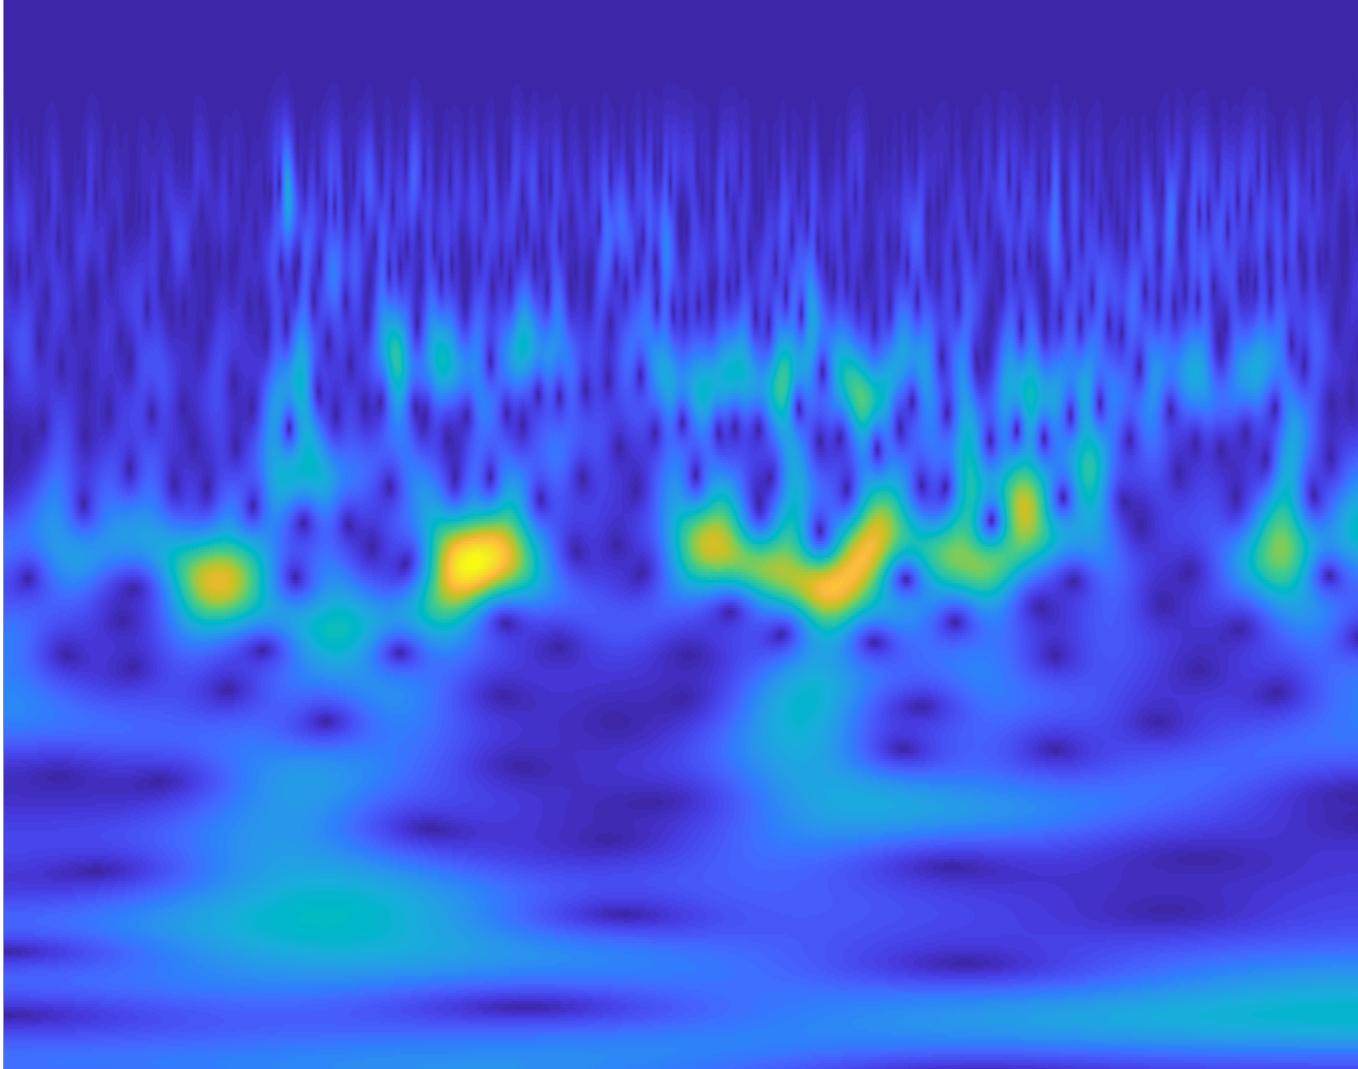
\includegraphics[width=12cm,height=6.5cm]{cwt.png}};
%%%%%%%%%%%%%%%%%%%%%%%%%%%%%%%%%%%%%%%%%%%%%%%%%%%%%%%%%%%%%%%%%%%%%%%%%%%%%%%%%%%%%%%%
%% Draw Arrow Connections
%%%%%%%%%%%%%%%%%%%%%%%%%%%%%%%%%%%%%%%%%%%%%%%%%%%%%%%%%%%%%%%%%%%%%%%%%%%%%%%%%%%%%%%%
\draw [connection]  (tc1-east)       -- node {\midarrow} (tc2-west);
\draw [connection]  (tc2-east)       -- node {\midarrow} (rz1-west);
\draw [connection]  (rz1-east)       -- node {\midarrow} (tc3-west);
\draw [connection]  (tc3-east)       -- node {\midarrow} (tc4-west);
\draw [connection]  (tc4-east)       -- node {\midarrow} (rz2-west);
\draw [connection]  (rz2-east)       -- node {\midarrow} (tc5-west);
\draw [connection]  (tc5-east)       -- node {\midarrow} (tc6-west);
\draw [connection]  (tc6-east)       -- node {\midarrow} (rz3-west);
\draw [connection]  (rz3-east)       -- node {\midarrow} (lgt-west);
%%%%%%%%%%%%%%%%%%%%%%%%%%%%%%%%%%%%%%%%%%%%%%%%%%%%%%%%%%%%%%%%%%%%%%%%%%%%%%%%%%%%%%%%
%% Draw Dotted Edges 
%%%%%%%%%%%%%%%%%%%%%%%%%%%%%%%%%%%%%%%%%%%%%%%%%%%%%%%%%%%%%%%%%%%%%%%%%%%%%%%%%%%%%%%%
% \draw[densely dashed]
% (rz3-west)++(0, 1.5*.2, 1.5*.2) coordinate(a) -- (outputs-nearnortheast)
% (rz3-west)++(0,-1.5*.2, 1.5*.2) coordinate(b) -- (outputs-nearsoutheast)
% (rz3-west)++(0,-1.5*.2,-1.5*.2) coordinate(c) -- (outputs-farsoutheast)
% (rz3-west)++(0, 1.5*.2,-1.5*.2) coordinate(d) -- (outputs-farnortheast)

% (a)--(b)--(c)--(d)
% ;
%%%%%%%%%%%%%%%%%%%%%%%%%%%%%%%%%%%%%%%%%%%%%%%%%%%%%%%%%%%%%%%%%%%%%%%%%%%%%%%%%%%%%%%%
\end{tikzpicture}
\end{document}